\chapter{Results}
\label{chap:results}


Spatially and spectrally resolved line emission was detected for CO (3-2), HCO$^{+}$ (4-3), HCN (4-3), and CS (7-6) across around 50 channels of width 0.42 km s$^{-1}$. Here we present a discussion of these data, including line-emission statistics, diagnostic plots, and a consideration of the cloud contamination present.


Here are presented line-emission statistics, as well as moment maps, channel maps, and a discussion on the role of cloud contamination in the data.


\bigskip

\section{Cloud Contamination}
\label{section:cloud_contamination}
% Ex footnote: \texttt{K2Phot}\footnote{\href{https://github.com/vincentvaneylen/k2photometry}{https://github.com/vincentvaneylen/k2photometry}} \citep{vaneylen2016}

Cloud contamination occurs when emission from gas clouds along the observation's line of sight is detected. This is typically not a significant issue for observations of proplyds in low-mass star forming regions (SFRs), but since the Orion Nebula has a signicantly higher gas density than those low-mass SFRs, cloud contamination presents problems in these data. This is particularly evident in the CO line, thanks to its low critical density and relatively high abundance in the background clouds, which allows it to excite and emit more readily than other molecules. As a result of higher critical densities and lower abundances, cloud contamination is less significant, but still present, in the other lines. It is crucial to manage and minimize the effects of this contamination before modeling so that our fitting algorithms do not try to model the cloud emission.

% You’ll need to explain why we want to minimize rms noise: normally, removing data should increase rms noise (because rms noise should decrease as the square root of the number of data points).  However, when we remove short baselines we see exactly the opposite, which tells us that there is signal on the short baselines (from the cloud) causing the off-source rms to be artificially inflated.  We look for the inflection point where the plot goes from decreasing rms noise to increasing rms noise, because that tells us that noise statistics are starting to dominate over cloud contamination. 



Luckily, there exist ways to minimize the effects of cloud contamination. To do so, we take advantage of the fact that the contaminating clouds tend to be very large relative to a proplyds and that, as discussed in \S\ref{chapter:introduction}, interferometers have the ability to filter by length scale. Using these two features, we may exclude a selection of the shortest baselines used in our data, effectively shrinking the largest angular scales and, consequently, significantly reducing the effects of the cloud emission.

%While this process slightly reduces the total recovered flux from the disks, that loss is far outweighed by the improvements in image cleanliness that we receive in exchange.

To see whether or not we have cloud contamination, we may make a plot of RMS-noise against shortest baseline (by iteratively removing more and more of the short baselines). Were there no cloud contamination, we would find that this plot trends upwards (following the fact that noise is typically proportional to the inverse square root of amount of data). However, we can recognize the signature of cloud contamination if we find unexpectedly high noise at low baselines that falls off at longer ones. This decrease reflects the fact that, since the clouds are large, only the shortest baselines are significantly affected. This indicates that the ideal value to use as our minimum baseline length would be the inflection point at which the cloud contamination's contribution (decreasing with baseline length) gives way to the normal losses that come with decreasing signal (increasing with baseline length)\footnote{Another way to justify the removal of data is to recall that, not only are these short baselines recording too much cloud emission, but they are also generally not sensitive to the disks, since they are too small for these short baselines to pick up. Therefore, losing them effectively removes noise without any consequence to the data we really care about.}. The results of making such plots are shown in Fig. \ref{fig:noise-profiles}.
% REWORK ^^

From these plots, we find that excluding baselines less than 110 k$\lambda$, 80 k$\lambda$, and 60  k$\lambda$ for HCO$^{+}$, HCN, and CO, respectively, yielded optimum results. Since emission from the CS line already has a very low SNR and a higher critical density than the clouds can easily access, it showed minimal contamination and thus excluding baselines did not improve the observations. Image statistics resulting from these cuts are presented in Table \ref{baseline_cutting_table}.

%REWORK: GET THE FUCKING IMAGE STATS


% Calculations for this are made in scratch_02.py but maybe should be in scratch_03 now.


\begin{table}
  \begin{threeparttable}
    \centering
    \caption{Integrated Flux Measurements with Baseline Cuts}
    \label{tab:baseline_cutting_table}
    \renewcommand{\arraystretch}{1.2}
    \begin{tabular}{l | c | c | c | c }
      \toprule \toprule
      Molecular       & Baselines       & Max Angular & \multicolumn{2}{c}{Integrated Line Flux (Jy km s$^{-1}$)} \\
      Line            & ncluded         & Scale       & Disk A        & Disk B \\
      \midrule %\midrule
      CS (7-6)        & All             & 8.\farcs5        & 0.024$\pm$ 0.02 & [no detection] \\
      CO (3-2)        & All             & 8.\farcs4        & [\tnote{*}] &  [\tnote{*}] \\
      CO (3-2)        & $>60 k\lambda$  & 3.\farcs4        & 2.58$\pm$ 0.47 & 1.85 $\pm$ 0.39 \\
      HCN (4-3)       & All             & 8.\farcs2        & 0.80$\pm$ 0.07 &  0.26 $\pm$ 0.08 \\
      HCN (4-3)       & $>80 k\lambda$  & 2.\farcs6        & 0.69$\pm$ 0.05 &  0.17 $\pm$ 0.08 \\
      HCO$^{+}$ (4-3) & All             & 8.\farcs2        & 5.79$\pm$ 0.49 &  2.29 $\pm$ 0.56 \\
      HCO$^{+}$ (4-3) & $>110 k\lambda$ & 1.\farcs9        & 4.15$\pm$ 0.31 &  0.80 $\pm$ 0.22 \\
      \bottomrule
    \end{tabular}
    \begin{tablenotes}\footnotesize
      \item[*] Integrated line intensity was not calculated for CO(3-2) before the baseline cuts, as the data were too contaminated to give meaningful results.
    \end{tablenotes}
  \end{threeparttable}
\end{table}

% Results from tools.py/get_int_line_flux()
% HCO+, >110: 0.62,
% HCO+, all: 0.80, 5.79(0.488), 2.287(0.561)
% CO, all: 0.51: unusable
% CO, >60: 0.495, 2.579(0.472), 1.855(0.391)
% HCN, all: 0.161, 0.797(0.0673), 0.255(0.077879)
% HCN, >80, 0.132, 0.690(0.0487), 0.170(0.0775)
% CS, all: 0.023, 0.0242(0.0246), NA




% NOISE PROFILES
% REWORK: Make this in one plot, with rows by line and cols by RMS/mean.
\begin{figure}
  \centering
  \begin{minipage}{.48\textwidth}
    \centering
    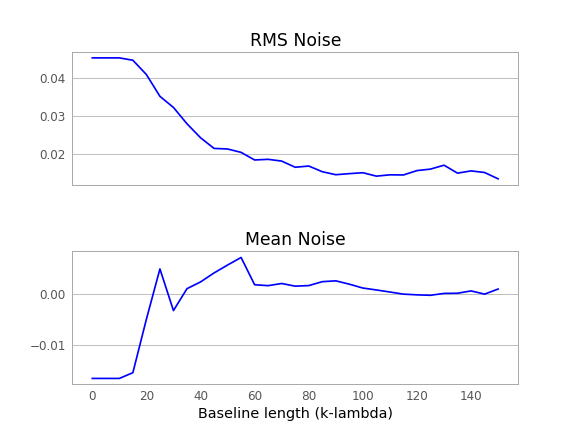
\includegraphics[width=\linewidth]{hco-imnoise_hco10000.png}
    \captionof{figure}{HCO$^+$ Noise profiles}
    \label{fig:noise-profile_hco}
  \end{minipage}%
  \begin{minipage}{.48\textwidth}
    \centering
    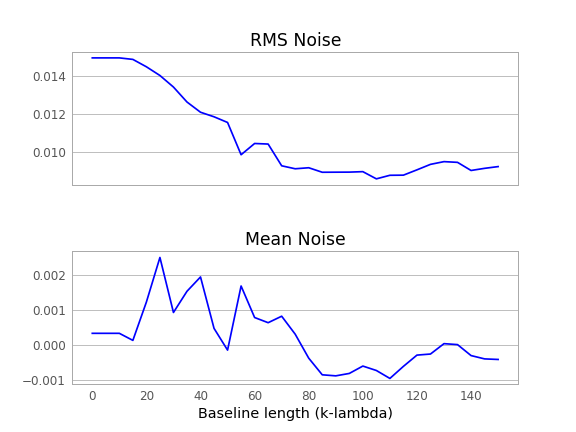
\includegraphics[width=\linewidth]{hcn-imnoise_hcn10000.png}
    \captionof{figure}{HCN Noise profiles}
    \label{fig:noise-profile_hcn}
  \end{minipage}%
  \par\medskip
  \begin{minipage}{.48\textwidth}
    \centering
    \includegraphics[width=\linewidth]{co-imnoise_co.png}
    \captionof{figure}{CO Noise profiles}
    \label{fig:noise-profile_co}
  \end{minipage}%
  \begin{minipage}{.48\textwidth}
    \centering
    \includegraphics[width=\linewidth]{cs-imnoise_cs.png}
    \captionof{figure}{CS Noise profiles}
    \label{fig:noise-profile_cs}
  \end{minipage}
  \label{fig:noise-profiles}
\end{figure}





\section{Line Data}
\label{section:line_data}

% REWORK: This feels clunky
% REWORK: Replot m0 and m1 maps to get the text on top.
Moment maps offer us ways to flatten the three-dimensional data-cube (in $v, \alpha, \delta$) into two dimensions. Moment 0 maps integrate flux along the velocity axis as a function of position, providing insight into structures of emission intensity in the disk's morphology, while moment 1 maps, a velocity-weighted intensity integration across position, present a source's velocity gradients. Figures \ref{fig:CO_m0} and \ref{fig:CO_m1} show zeroth- and first-moment maps, respectively, of the CO line emission, with and without a 60 k$\lambda$ baseline cut made (left and right, respectively).

% MOMENT MAPS
% REWORK: Maybe have vmin=-vmax for these plots?
\begin{figure}
\centering
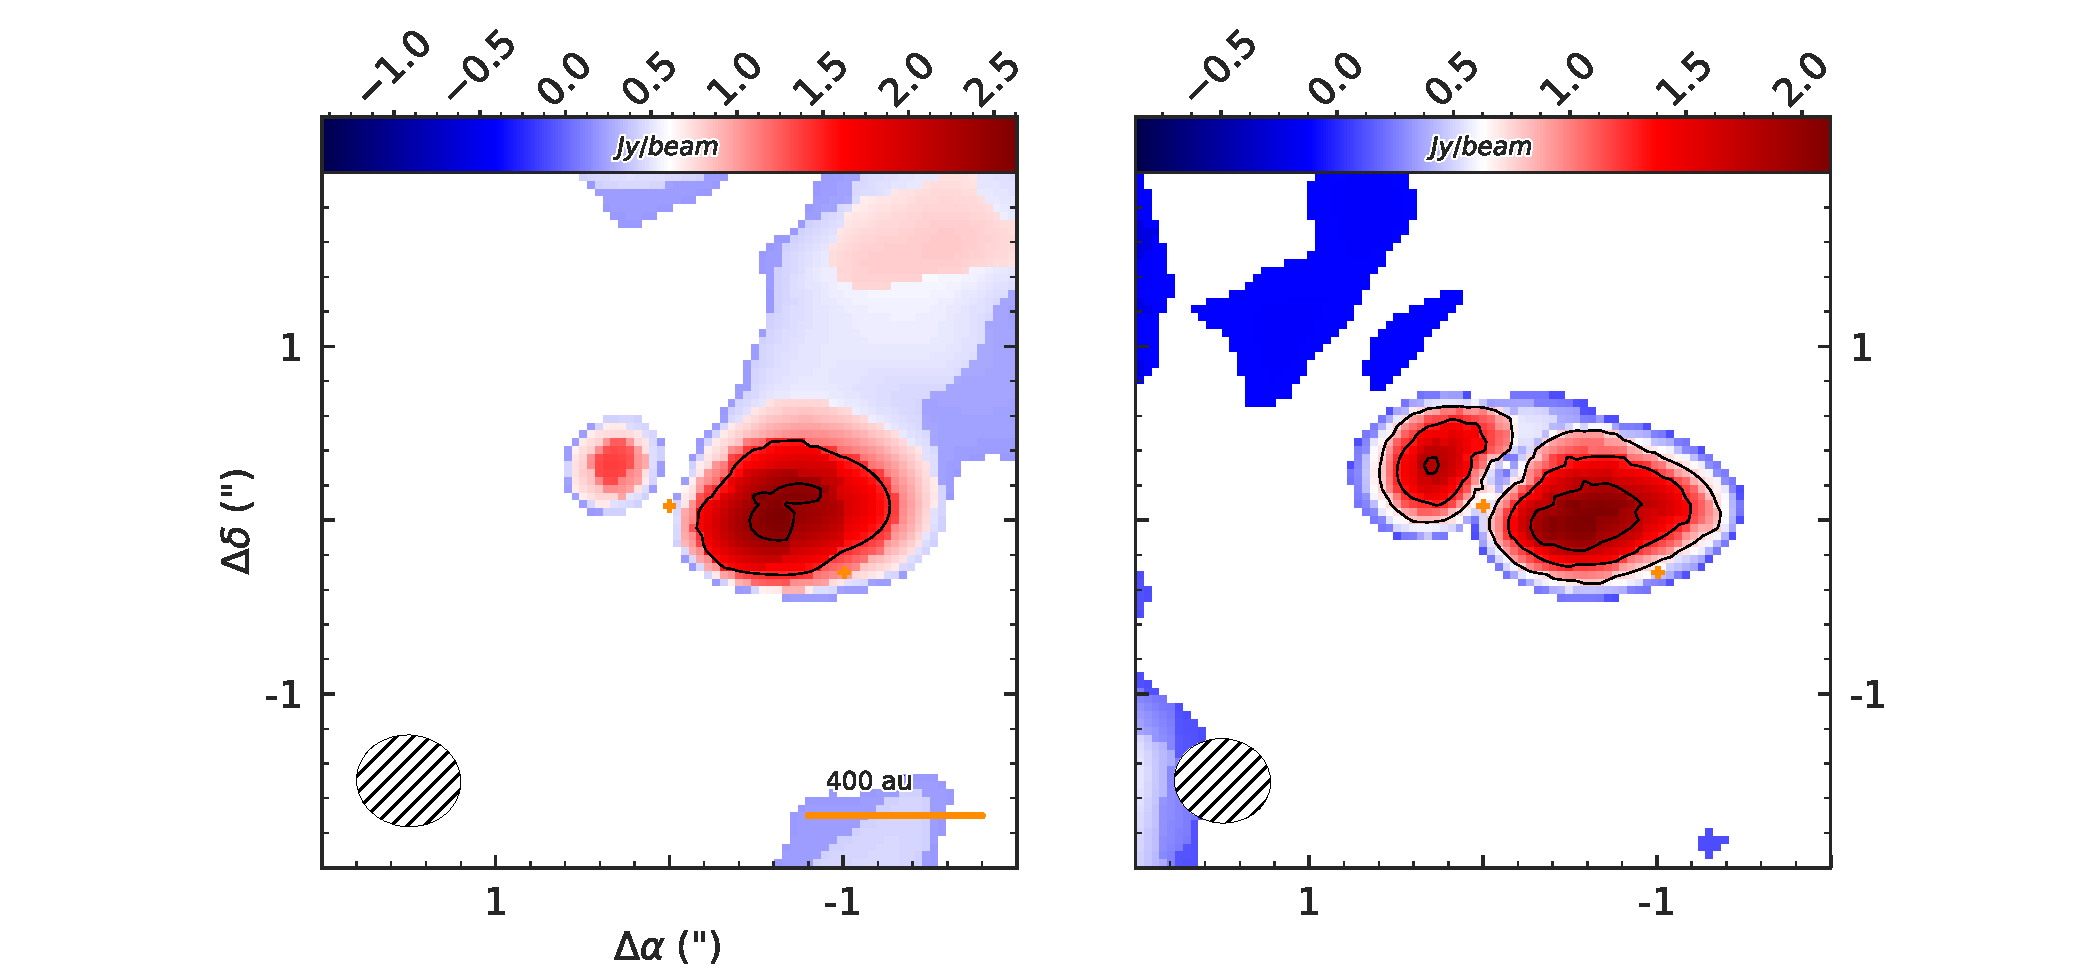
\includegraphics[width=\linewidth]{m0-map_co-co.pdf}[h!]
  \captionof{figure}{Zeroth moment map of CO emission, with and without a cut of all baseline's below 60 k$\lambda$ (left and right, respectively). Colors correspond to velocity-integrated intensity, while contours represent $\pm$3, 5, 7...15-$\sigma$ transitions where 1$\sigma$ is 0.257 Jy beam$^{-1}$ km s$^{-1}$. Negative contours are dashed. The beam is shown in the bottom left corner, with a diameter of 0."5 which corresponds to 200 AU at 389 parsec.}
  \label{fig:CO_m0}
  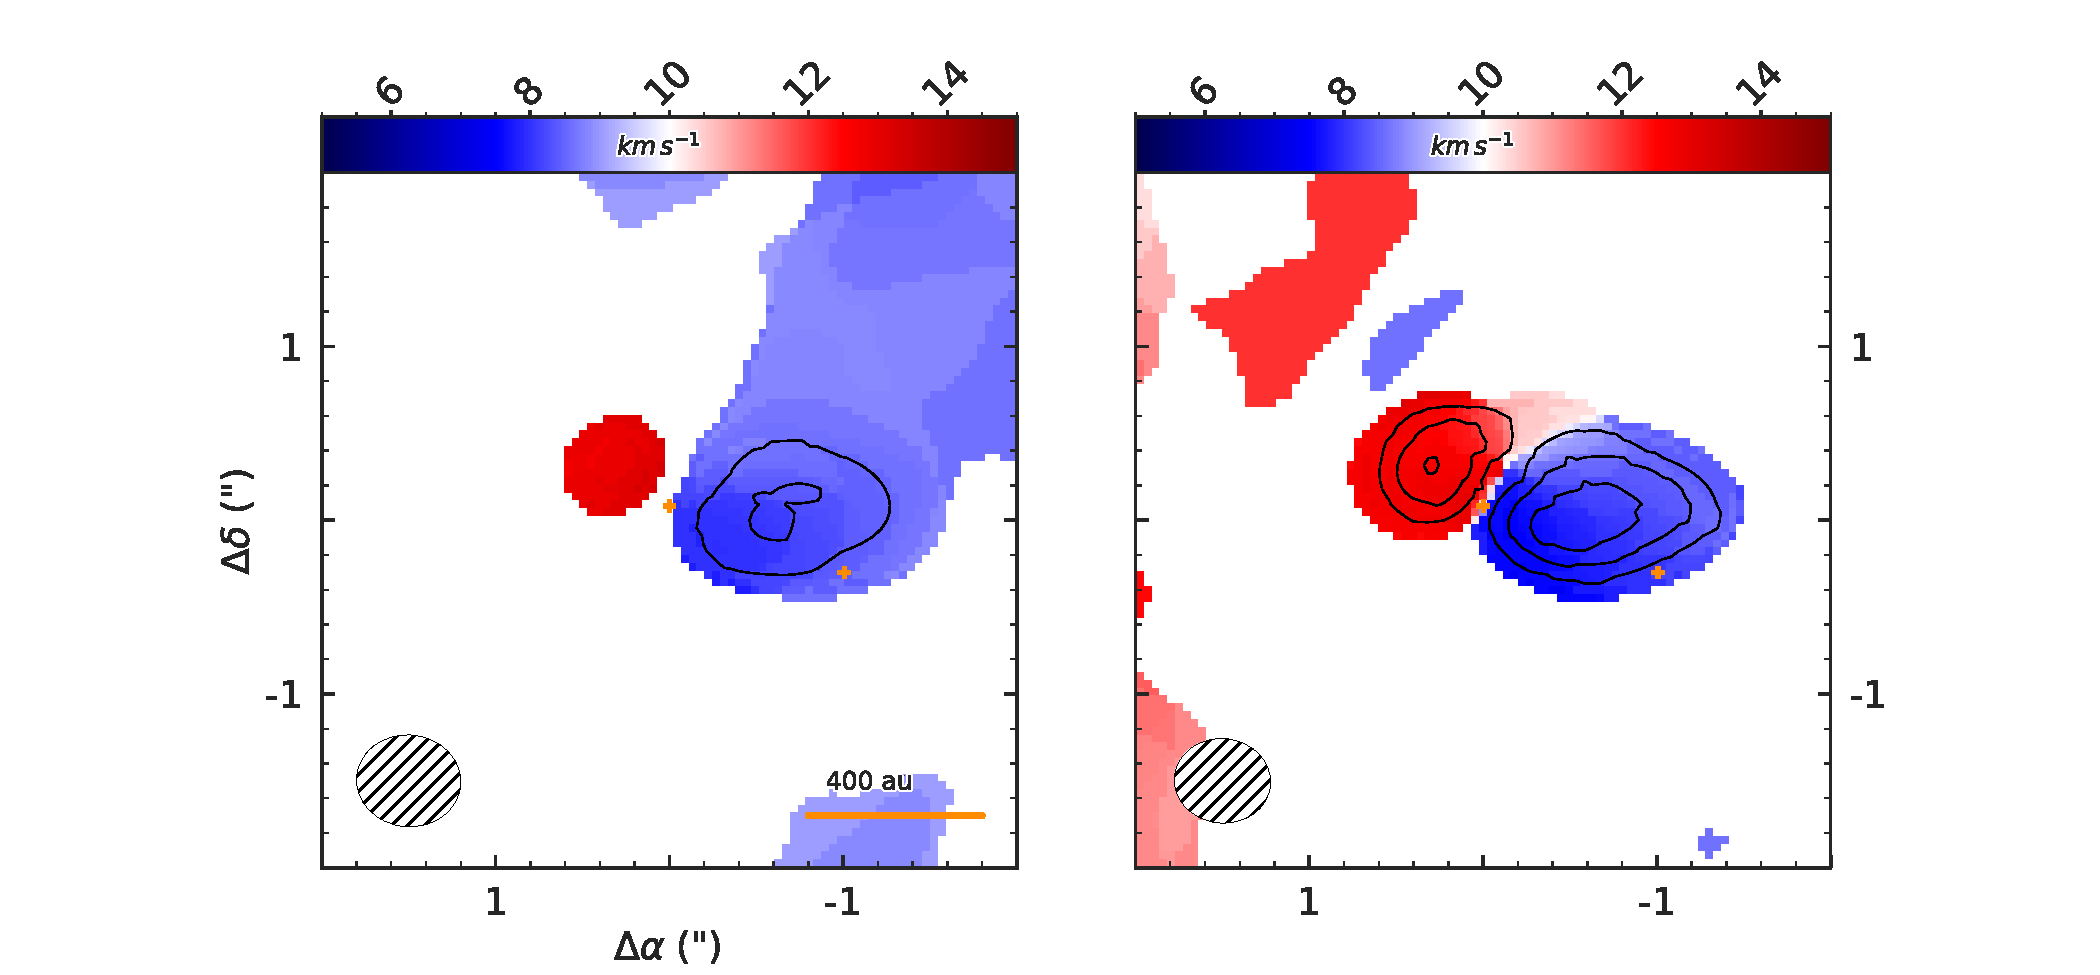
\includegraphics[width=\linewidth]{m1-map_co-co.pdf}
  \captionof{figure}{First moment map of CO emission, with and without a cut of all baseline's below 60 k$\lambda$ (left and right, respectively). Colors correspond to intensity-weighted LSRK velocity, while contours represent $\pm$3, 5, 7,..., 15-$\sigma$ transitions where 1$\sigma$ is 0.257 Jy beam$^{-1}$ km s$^{-1}$}
  \label{fig:CO_m1}
\end{figure}




Integrated line flux was measured using the Miriad task \texttt{cgcurs} to spatially integrate flux in a zeroth moment map over the region enclosed by the 3$\sigma$ contour. The results of these measurements are shown in \ref{baseline_cutting_table}. From these values, we may estimate the disks' gas masses.

Assuming optically thin emission and Local Thermodynamic Equilibrium (LTE), the line-emitting gas mass, M$_{\text{gas}}$ is given by:

\begin{align}
  M_{\text{gas}}= \frac{4 \pi}{h \nu_0} \frac{F m d^2}{A_{ul} X_u},
  \label{M_gas}
\end{align}

where $F$ is the integrated line flux, $m$ is the mass of the emitting gas molecule, $d$ is the distance to the source, $h$ is the Planck constant, $\nu_0$ is the molecular line's rest frequency, $A_{ul}$ is the Einstein coefficient for the ($u - l$) transition, and

\begin{align}
  X_u = \frac{N_u}{N_{\text{tot}}} = (2 J_u + 1) \frac{\exp [-B_0 J_u (J_u + 1) h c/kT_{\text{ex}}]}{kT_{\text{ex}}/hc B_0}.
  \label{X_u}
\end{align}

In Eqn. \ref{X_u}, $\frac{N_u}{N_{\text{tot}}}$ is the ratio of the number of molecules in the upper state to the total number of molecules; $J_u$ is the quantum number of the upper level; $B_0$ is the rotation constant in units of wavenumber; $h$ and $c$ are the Planck constant and speed of light, respectively; and $T_{\text{ex}}$ is the excitation temperature. Values for $A_{ul}$ and $B_0$ were taken from molecular data drawn from \citet{Schoeier2005}. The values used for this measurement are given in Table \ref{mass_calc_vals}. Since Eqn. \ref{M_gas} is the mass of the observed gas species, it must be scaled by the it's relative abundance (fit for in Section 4) to obtain a total mass (\textit{I'm not totally clear on this}). From this, we find a total mass of $0.x \pm 0.y M_{\odot}$.


\begin{table}
  \centering
  \begin{threeparttable}
    \caption{Values Used in Gas Mass Calculation (HCO$^+$)}
    \label{tab:baseline_cutting_table}
    \renewcommand{\arraystretch}{1.2}
    \begin{tabular}{l | c | c }
      \toprule \toprule
      Parameter   & Value       & Max Source  \\
      \midrule %\midrule
      F        & 4.15 Jy km s$^{-1}$   & Integrated line flux \\
      J        & 4             & NA \\
      A$_{4-3}$  & 0.363            & \citet{Schoeier2005}  \\
      E$_{4-3}$      & 29.75 cm$^{-1}$  & \citet{Schoeier2005} \\
      B$_0$        & All            & B$_0 = E_{4-3}/(\hbar c)$  \\
      T$_\text{excite}$        & All             & 8.\farcs4  \\
      Distance        & All             & 8.\farcs4  \\
      B$_0$        & All             & 8.\farcs4  \\
      \bottomrule
    \end{tabular}
    \begin{tablenotes}\footnotesize
      \item[*] Integrated line intensity was not calculated for CO(3-2) before the baseline cuts, as the data were too contaminated to give meaningful results.
    \end{tablenotes}
  \end{threeparttable}
\end{table}




A Position-Velocity (PV) diagram of the disk A's \hco emission is presented in \ref{fig:pv_diag}. The diagram shows the velocity distribution of of emission along a slice along the disk's major axis. There is some noticeable asymmetry in the emisison, both in terms of centroid intensity and in the extra feature at the eastern side of the map, which is likely the tail of disk B.

\note{I don't know how valuable these PV diagrams are - is just having this one, of one disk in one emission line, sufficient, or should I make them for both disks in HCO+/both disks in all lines/something else? At this point, they're fairly easy to make, so the main cost would just be clutter.}


\begin{figure}
  \centering
  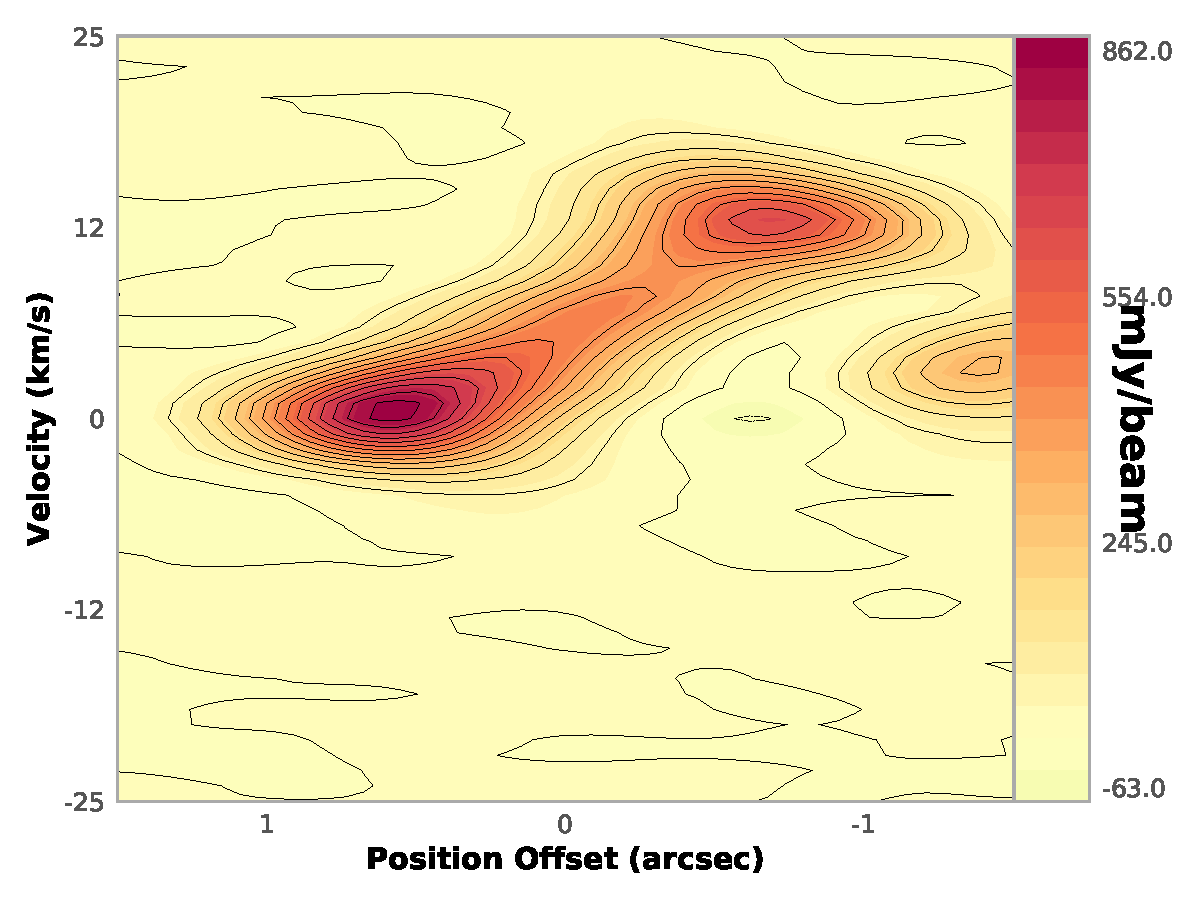
\includegraphics[width=\linewidth]{pvd_A.pdf}[h!]
    \captionof{figure}{A PV diagram of disk A's \hco emission. Some asymmetries are readily noticeable.}
    \label{fig:pv_diag}
\end{figure}






% Note that no closing info is needed.
